\section{Progress Report}

\subsection{Progress Status Overview}
For the January milestone, the project is progressing smoothly.
The Literature Review and Design Sections have been completed.
A working Version 1 prototype has been implemented. 
Student Struggle and Question Difficulty models have been developed
\subsection{Work Completed to Date}
The following work has been completed as part of the project:
\begin{itemize}
    \item A relevant literature review covering learning analytics, real-time dashboard and existing education systems
    \item Formulation of functional and non-functional system requirements
    \item Design of overall system architecture, including the data flow and component interactions
    \item Definitions of mathematical models for student struggle and question difficulty
    \item Implementation of Version 1 data pipeline using refreshing and session-level aggregation
    \item Development of a working instructor-facing dashboard prototype using Streamlit    
\end{itemize}
This work establishes a solid foundation for future work.

\subsection{Current Limitations}
The version 1 dashboard comes with a range of limitations:
\begin{itemize}
    \item Struggle is currently based on a single metric as a proof of concept
    \item AI Based classifications and question difficulty have not been implemented
    \item Data ingestion relies on refreshing rather than an event-driven architecture
    \item No task allocaiton to lab assistants
\end{itemize}

\subsection{Planned work}
The remaining work will focus on:
\begin{itemize}
    \item integrating the proposed analytics into the existing pipeline 
    \item replacing refresh ingestion logic with an event-driven logic.
    \item survey from both students and teachers
    \item Task allocation to lab assistants through smart devices
\end{itemize}

\subsection{Gantt Chart}

\begin{figure}[H]
    \centering
    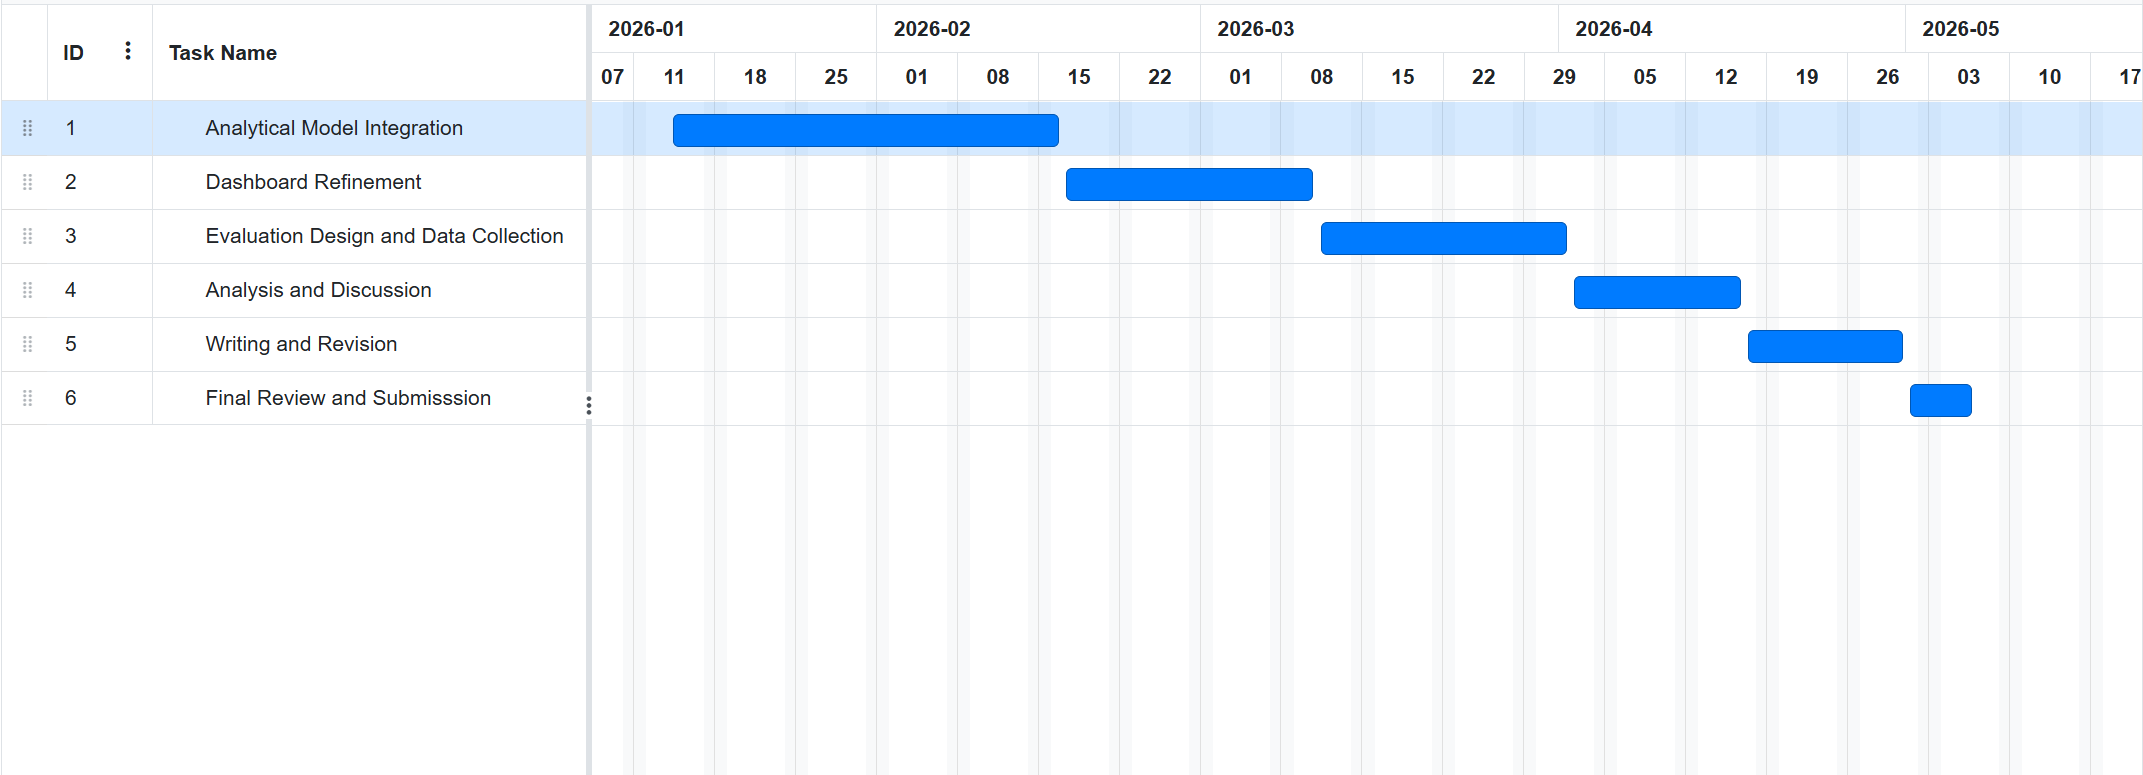
\includegraphics[width=1.2\textwidth]{figures/gantt.png}
    \caption{Project timeline from January 2026 to final submission in May 2026}
    \label{fig: Gantt}
\end{figure}


\begin{table}[H]
    \centering
    \begin{tabular}{|p{0.3\textwidth}|p{0.3\textwidth}|p{0.3\textwidth}|}
    \hline
       Task  & Start Date & End Date \\
    \hline
    \hline
       Analytical Model Integration  & 14/1/26 & 16/2/26\\
    \hline
        Dashboard Refinement & 17/2/26 & 10/3/26\\
    \hline
        Evaluation Design and Data Collection & 11/3/26 & 1/4/26\\
    \hline
        Analysis and Discussion& 2/4/26 & 16/4/26\\
    \hline
         Writing and Revision& 17/4/26 & 30/4/26\\
    \hline
         Final Review and Submission & 1/5/26 & 6/5/26\\
    \hline

    \end{tabular}
    \caption{Summary table for what is in the Gantt Chart}
    \label{tab: gantt summary}
\end{table}